\section{R Turotium (17.05.2018, 24.05.2018) }
\begin{itemize}
\item[-]Führen Sie die im Tutorium: https://www.tutorialspoint.com/r/r\_web\_data.htm angegebenen Unterpunkte zu R Data Interfaces, R Charts \& Graphs und R Statistics Examples aus.
\item[-]Wenden Sie anschließend die Beispiele aus den Tutorien auf Ihre eigenen Daten an
\end{itemize}

\subsection*{Kurzdarstellung der Aufgabenstellung}
Es soll die grundlegende Funktionsweise von R verstanden werden durch die Anwendung oeffentlich zugänglicher Tutorials.

\subsection*{Lösung}
Als Dataset wurde die Bevoelkerungshistorie der einzelnen EU Laender nach Jahren zwischen 1960 und 2016 gewaehlt. 

\begin{itemize}
\item[-]Zuerst wird R-Studio gestartet

\item[-]Mittels folgendem Befehl ermittelt wir das working directory auf die R-Installation eingestellt ist(\autoref{fig:tutor1}):
\begin{figure}[!htb]
        \begin{minipage}{1\textwidth}
                \centering
                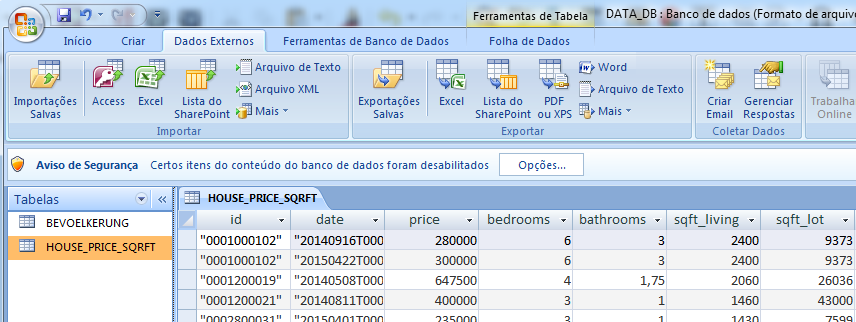
\includegraphics[width=0.50\textwidth]{pics/tutor1.png}\par\vspace{0cm}
                \caption{Standardpfad festlegen}
                \label{fig:tutor1}
        \end{minipage}
\end{figure}
	
\item[-]Die .csv Datei („BEVOELKERUNG.csv“)wird in den zuvor ermittelten Ordner gelegt

\item[-]Über den folgenden Befehl werden die Daten aus \\ „C:/Users/admin/Documents/BEVOELKERUNGSDATEN.csv“ in eine R variable geladen:
\begin{lstlisting}
data <- read.csv("BEVOELKERUNG.csv")
\end{lstlisting}
\item[-]Über diesen Befehl werden die ersten 6 Zeilen einer Variable ausgegeben werden(\autoref{fig:tutor2}):
\begin{figure}[!htb]
        \begin{minipage}{1\textwidth}
                \centering
                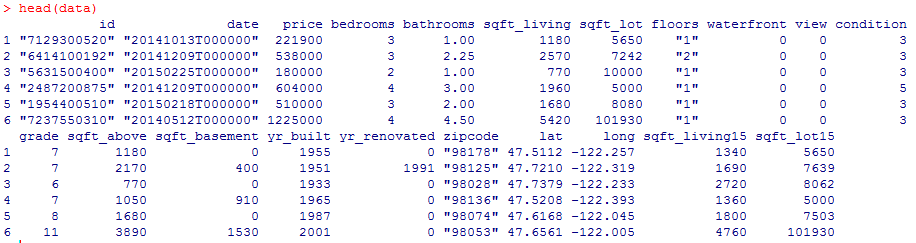
\includegraphics[width=0.50\textwidth]{pics/tutor2.png}\par\vspace{0cm}
                \caption{Anzeige der Zeilen}
                \label{fig:tutor2}
        \end{minipage}
\end{figure}

\section*{Tortendiagramm}
Zum Vergleich der Bevoelkerungsverteilung ueber die Laender der heutigen EU soll je ein Torten-Diagramm für 1996 und 2016 erstellt werden:

\subsection*{1966}
\item[-]Daten für 1966 muessen zuerst ein eine Variable separiert werden:
\begin{lstlisting}
J1966 <- data[ which(data$Jahr==1966), ]
\end{lstlisting}
\item[-]Ausgabe der ersten 6 Zeilen von J1966(\autoref{fig:tutor3}):
\begin{figure}[!htb]
        \begin{minipage}{1\textwidth}
                \centering
                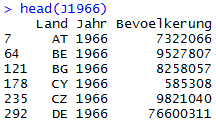
\includegraphics[width=0.50\textwidth]{pics/tutor3.png}\par\vspace{0cm}
                \caption{Ausgabe Variable}
                \label{fig:tutor3}
        \end{minipage}
\end{figure}

\item[-]Zum Erstellen des Diagramm werden zuerst die betreffenden Spalten in Variablen verwiesen mittels der folgenden beiden Befehle:
\begin{lstlisting}
x <- J1966$Bevoelkerung
labels <- J1966$Land
\end{lstlisting}
\item[-]Dateiname und Typ für die Diagramm-Ausgabe festlegen:
\begin{lstlisting}
png(file = "Bevoelkerung_1966.jpg")
\end{lstlisting}
			
\item[-]Plotten des Diagramms
\begin{lstlisting}
pie(x,labels, main = "Bevoelkerung 1966")
\end{lstlisting}

\item[-]Diagramm in zuvor angebene Datei ``Bevoelkerung\_1996.jpg`` speichern:
\begin{lstlisting}
dev.off()
\end{lstlisting}

\item[-]Fertiges Diagramm(\autoref{fig:tutor4}):
\begin{figure}[!htb]
        \begin{minipage}{1\textwidth}
                \centering
                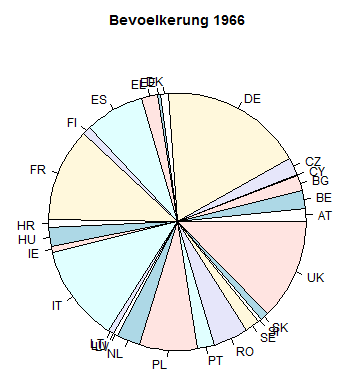
\includegraphics[width=0.50\textwidth]{pics/tutor4.png}\par\vspace{0cm}
                \caption{Bevölkerung 1966}
                \label{fig:tutor4}
        \end{minipage}
\end{figure}

\section*{2016}
\item[-]Daten für 2016 muessen zuerst ein eine Variable separiert werden:
\begin{lstlisting}
J2016 <- data[ which(data$Jahr==2016), ]		
\end{lstlisting}
		
\item[-]Ausgabe der ersten 6 Zeilen von J2016(\autoref{tutor5}):
\begin{figure}[!htb]
        \begin{minipage}{1\textwidth}
                \centering
                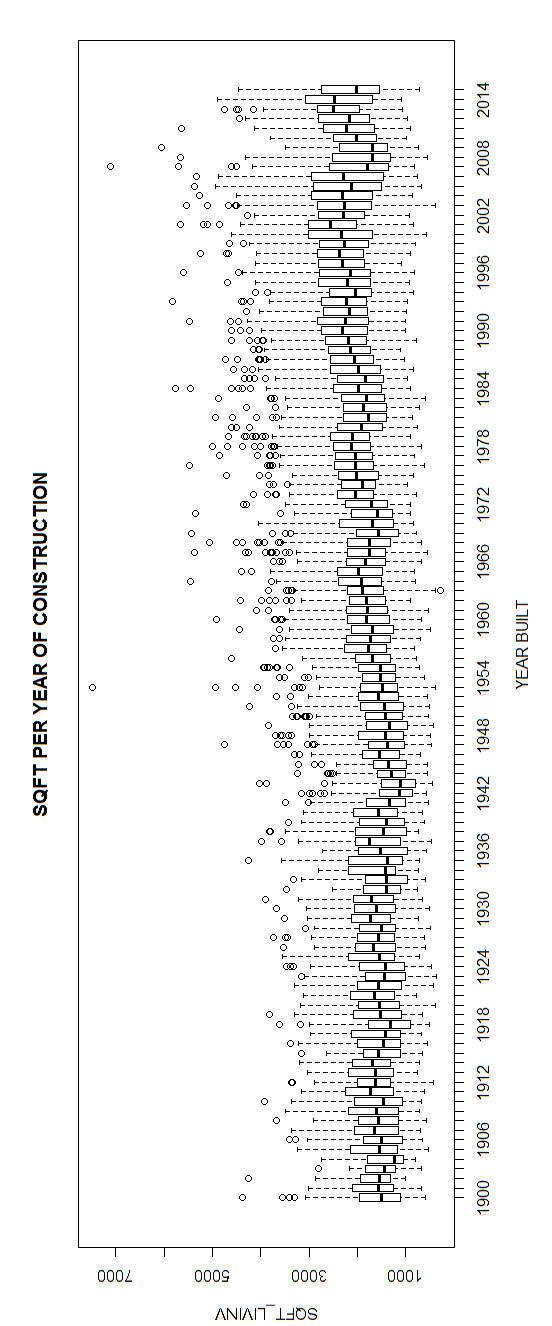
\includegraphics[width=0.50\textwidth]{pics/tutor5.png}\par\vspace{0cm}
                \caption{Variablenausgabe}
                \label{fig:tutor5}
        \end{minipage}
\end{figure}
\item[-]Zum Erstellen des Diagramm werden zuerst die betreffenden Spalten in Variablen verwiesen mittels der folgenden beiden Befehle:
\begin{lstlisting}
x <- J2016$Bevoelkerung
labels <- J2016$Land
\end{lstlisting}
\item[-]Dateiname und Typ für die Diagramm-Ausgabe festlegen:
\begin{lstlisting}
png(file = "Bevoelkerung_2016.jpg")
\end{lstlisting}
\item[-]Plotten des Diagramms
\begin{lstlisting}
pie(x,labels, main = "Bevoelkerung 2016")
\end{lstlisting}
\item[-]Diagramm in zuvor angebene Datei ``Bevoelkerung\_2016.jpg`` speichern:
\begin{lstlisting}
dev.off()
\end{lstlisting}
\item[-]fertiges Diagramm(\autoref{fig:tutor6}):
\begin{figure}[!htb]
        \begin{minipage}{1\textwidth}
                \centering
                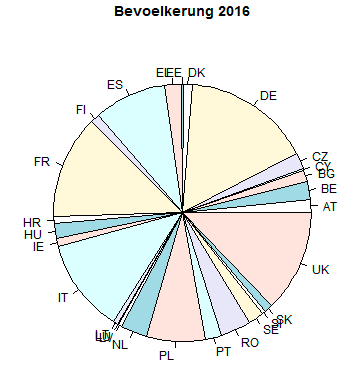
\includegraphics[width=0.50\textwidth]{pics/tutor6.png}\par\vspace{0cm}
                \caption{Bevölerung 2016}
                \label{fig:tutor6}
        \end{minipage}
\end{figure}

\section*{Bar-Charts}
\subsection*{Frankreich}
\item[-]Daten für Frankreich muessen zuerst ein eine Variable separiert werden:
\begin{lstlisting}
FR <- data[ which(data$Land=='FR'), ]
\end{lstlisting}
\item[-]Ausgabe der ersten 6 Zeilen von FR(\autoref{fig:tutor7}):
\begin{figure}[!htb]
        \begin{minipage}{1\textwidth}
                \centering
                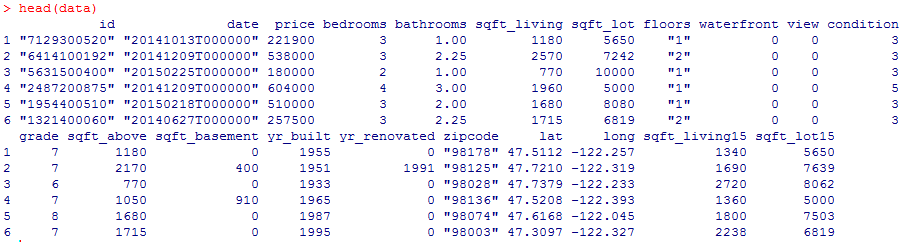
\includegraphics[width=0.50\textwidth]{pics/tutor7.png}\par\vspace{0cm}
                \caption{Zeilenausgabe}
                \label{fig:tutor7}
        \end{minipage}
\end{figure}
\item[-]Zum Erstellen des Diagramm werden zuerst die betreffenden Spalten in Variablen verwiesen mittels der folgenden beiden Befehle:
\begin{lstlisting}
Y <- FR$Bevoelkerung
X <- FR$Jahr
\end{lstlisting}
\item[-]Dateiname und Typ für die Diagramm-Ausgabe festlegen:
\begin{lstlisting}
png(file = "Bevoelkerunghistorie_Frankreich.png")
\end{lstlisting}
\item[-]Plotten des Diagramms
\begin{lstlisting}
barplot(Y,names.arg=X,xlab="Jahr",ylab="Bevoelkerung",col="blue",main="Bevoelkerungsentwicklung FR")
\end{lstlisting}
\item[-]Diagramm in zuvor angebene Datei ``Bevoelkerung\_2016.jpg`` speichern:
\begin{lstlisting}
dev.off()
\end{lstlisting}
\item[-]fertiges Diagramm(\autoref{fig:tutor8}):

\begin{figure}[!htb]
        \begin{minipage}{1\textwidth}
                \centering
                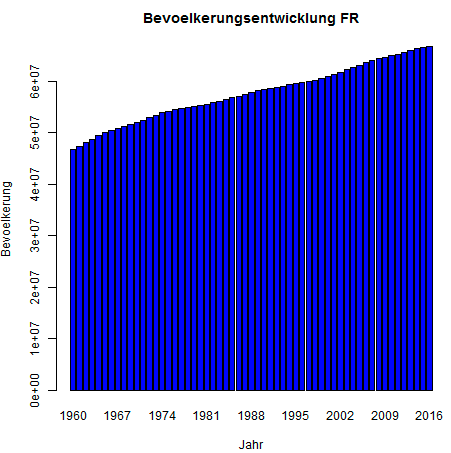
\includegraphics[width=0.50\textwidth]{pics/tutor8.png}\par\vspace{0cm}
                \caption{Diagramm: Frankreich}
                \label{fig:tutor8}
        \end{minipage}
\end{figure}

\section*{Deutschland}
\item[-]Daten für Deutschland muessen zuerst ein eine Variable separiert werden:
\begin{lstlisting}
DE <- data[ which(data$Land=='DE'), ]
\end{lstlisting}
\item[-]Ausgabe der ersten 6 Zeilen von de(\autoref{fig:tutor9}):
\begin{figure}[!htb]
        \begin{minipage}{1\textwidth}
                \centering
                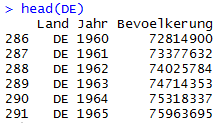
\includegraphics[width=0.50\textwidth]{pics/tutor9.png}\par\vspace{0cm}
                \caption{Variablenverwendung}
                \label{fig:tutor9}
        \end{minipage}
\end{figure}
\item[-]Zum Erstellen des Diagramm werden zuerst die betreffenden Spalten in Variablen verwiesen mittels der folgenden beiden Befehle:
\begin{lstlisting}
Y <- DE$Bevoelkerung
X <- DE$Jahr
\end{lstlisting}

\item[-]Dateiname und Typ für die Diagramm-Ausgabe festlegen:
\begin{lstlisting}
png(file = "Bevoelkerunghistorie_Deutschland.png")
\end{lstlisting}
\item[-]Plotten des Diagramms
\begin{lstlisting}
barplot(Y,names.arg=X,xlab="Jahr",ylab="Bevoelkerung",col="blue",main="Bevoelkerungsentwicklung DE")
\end{lstlisting}
\item[-]Diagramm in zuvor angebene Datei ``Bevoelkerung\_2016.jpg`` speichern:
\begin{lstlisting}
dev.off()
\end{lstlisting}
\item[-]fertiges Diagramm(\autoref{fig:tutor10}):
\begin{figure}[!htb]
        \begin{minipage}{1\textwidth}
                \centering
                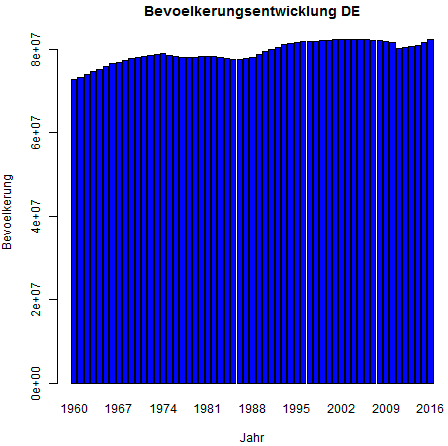
\includegraphics[width=0.50\textwidth]{pics/tutor10.png}\par\vspace{0cm}
                \caption{Bevölkerungsentwicklung DE}
                \label{fig:tutor10}
        \end{minipage}
\end{figure}
\end{itemize}
\subsection*{Aufteilung der Aufgaben im Team}
Alle Aufgabenpunkte wurden gemeinsam bearbeitet
\subsection*{Darstellung der benutzen Werkzeuge und Systeme}
\subsubsection*{Entwurfswerkzeug}
R-Studio
\subsubsection*{Entwicklungsumgebung}
R-Studio

